\documentclass[a4paper,10pt]{article}
\usepackage{amsmath,amssymb,graphicx,float,subfig}

%defines
\def\bY{{\bf Y}}
\def\bX{{\bf X}}
\def\bE{{\bf E}}
\def\bV{{\bf V}}
\def\bC{{\bf C}}
\def\b1{{\bf 1}}
\def\bx{{\bf x}}
\def\blambda{{\boldsymbol \lambda}}
\def\bgamma{{\boldsymbol \gamma}}
\def\bbeta{{\boldsymbol \beta}}
\def\bnu{{\boldsymbol \nu}}
\def\bmu{{\boldsymbol \mu}}
\def\sigmaeps{{\sigma_{\epsilon}}}

%opening
\title{Home Assignment - 1}
\author{Santhosh Nadig, Zhanzhang Cai}

\begin{document}

\maketitle

\section{Introduction}
Spatially consecutive temperature data is an important evaluating criterion of global/regional climate model and a pivotal driver of dynamic vegetation model. In spatial statistics, a common situation is to reconstruct (interpolate) values at unobserved locations from observations at some measurement locations. In this assignment, we will reconstruct average monthly temperature for Sweden during June of 2005, using observations from weather stations. Ordinary least squares and universal Kriging will be tested for their performance in reconstructing the monthly average temperature at the validation sites and on the prediction grid.
\section{Theory}
Let $\bY_k$ represent the $n$ known observations of spatial data and $\bY_u$ represent the $m$ data points that needs to be estimated. For ordinary Kriging ($\mu = \b1 \beta$), the optimal predictions are given by
\begin{align*}
 \hat \bY_u &= \b1_u \hat \beta + \Sigma_{uk} \Sigma_{kk}^{-1}\left( \bY_k - \b1_k \hat \beta \right) \\
 \hat \beta &= \left( \b1_k^T \Sigma_{kk}^{-1} \b1_k \right)^{-1} \b1_k^T \Sigma_{kk}^{-1} \bY_k,
\end{align*}
where
\begin{align*}
 &\begin{bmatrix}
  \bY_k \\
  \bY_u
 \end{bmatrix} \in
 \mathbf{N} \left( 
 \begin{bmatrix}
    \b1_k \beta \\
   \b1_u \beta
  \end{bmatrix},
  \begin{bmatrix}
   \Sigma_{kk} & \Sigma_{ku} \\
   \Sigma_{uk} & \Sigma_{uu}
  \end{bmatrix}
  \right).
\end{align*}

Firstly, we show that the predictions are linear in the observations, i.e., $\hat \bY_u = \blambda^T \bY_k$ for some $\blambda$. We may re-write $\hat \beta$ as
\begin{align*}
 \hat \beta &= \bgamma^T \bY_k \\
 \bgamma &= \left( \left( \b1_k^T \Sigma_{kk}^{-1} \b1_k \right)^{-1} \b1_k^T \Sigma_{kk}^{-1} \right)^T.
\end{align*}
We note that the vector $\bgamma^T$ is of dimensions $1 \times n$, and therefore, $\hat \beta$ is a scalar. Substituting the above in the expression for $\hat \bY_u$, we obtain
\begin{align*}
 \hat \bY_u &= \b1_u \bgamma^T \bY_k + \Sigma_{uk} \Sigma_{kk}^{-1} \bY_k -  \Sigma_{uk} \Sigma_{kk}^{-1}  \b1_k \bgamma^T \bY_k \\
      &= \left( \b1_u \bgamma^T + \Sigma_{uk} \Sigma_{kk}^{-1} -  \Sigma_{uk} \Sigma_{kk}^{-1}  \b1_k \bgamma^T \right) \bY_k \\
      &= \blambda^T \bY_k,
\end{align*}
where $\blambda = \left( \b1_u \bgamma^T + \Sigma_{uk} \Sigma_{kk}^{-1} -  \Sigma_{uk} \Sigma_{kk}^{-1}  \b1_k \bgamma^T \right)^T$.

Secondly, we show that the predictions are unbiased, i.e., $\bE(\hat \bY_u) = \bE(\bY_u)$. The expected value of $\hat \beta$ is given by
\begin{align*}
 \bE \left( \hat \beta \right) &= \left( \b1_k^T \Sigma_{kk}^{-1} \b1_k \right)^{-1} \b1_k^T \Sigma_{kk}^{-1} ~ \bE (\bY_k) \\
  &= \left( \b1_k^T \Sigma_{kk}^{-1} \b1_k \right)^{-1} \b1_k^T \Sigma_{kk}^{-1} ~ \b1_k \beta \\
  &= \beta.
\end{align*}
Therefore,
\begin{align*}
 \bE(\hat \bY_u) &=  \b1_u \bE\left(\hat \beta \right) + \Sigma_{uk} \Sigma_{kk}^{-1}\left( \bE(\bY_k) - \b1_k \bE \left(\hat \beta \right)\right) \\
 &= \b1_u \beta + \Sigma_{uk} \Sigma_{kk}^{-1}\left( \b1_k \beta - \b1_k \beta \right) \\
 &= \b1_u \beta.
\end{align*}

Finally, consider a second unbiased predictor of $\bY_u$, given by $\tilde \bY_u = (\blambda + \bnu)^T \bY_k$. From the unbiasedness criterion, we have that $\bE(\tilde \bY_u) = \bE(\hat \bY_u)$. Therefore, $(\blambda + \bnu)^T \bE(\bY_k) = \blambda^T \bE(\bY_k)$, implying $\bnu^T \b1_k = 0$. Furthermore, consider the variance of the second predictor
\begin{align*}
 \bV(\tilde \bY_u - \bY_u) &= \bV(\bnu^T \bY_k + (\blambda^T \bY_k - \bY_u))\\
 &= \bV(\bnu^T \bY_k) + \bV(\hat \bY_u - \bY_u) + 2\bC(\bnu^T \bY_k, \hat \bY_u - \bY_u) \\
 &\ge \bV(\hat \bY_u - \bY_u) + 2\bC(\bnu^T \bY_k, \hat \bY_u - \bY_u)\\
 &= \bV(\hat \bY_u - \bY_u) + 2\bnu^T \bC(\bY_k, \hat \bY_u) - 2 \bnu^T \bC(\bY_k, \bY_u) \\
 &= \bV(\hat \bY_u - \bY_u) + 2\bnu^T \left(  \Sigma_{kk} \blambda - \Sigma_{uk}\right)
\end{align*}
Thus, if we can choose $\blambda$ such that $\bnu^T \left(  \Sigma_{kk} \blambda - \Sigma_{uk}\right) = 0$, then, we have that $\bV(\tilde \bY_u - \bY_u) \ge \bV(\hat \bY_u - \bY_u)$ for any unbiased predictor $\tilde \bY_u$.

\section{Swedish Temparature Reconstruction}
The data consists of average temperature during June 2005 measured at 250 stations across Sweden. In addition, the latitude, longitude, elevation and distance to both the Swedish coast and to any coastline are provided too. Figure \ref{fig:rawdataplot} shows the plot of average temperature, elevation and distance to any coast. The average temperatures are higher in the South (lower latitudes) and towards the coast, as expected.
\begin{figure}[ht]
	\centering
	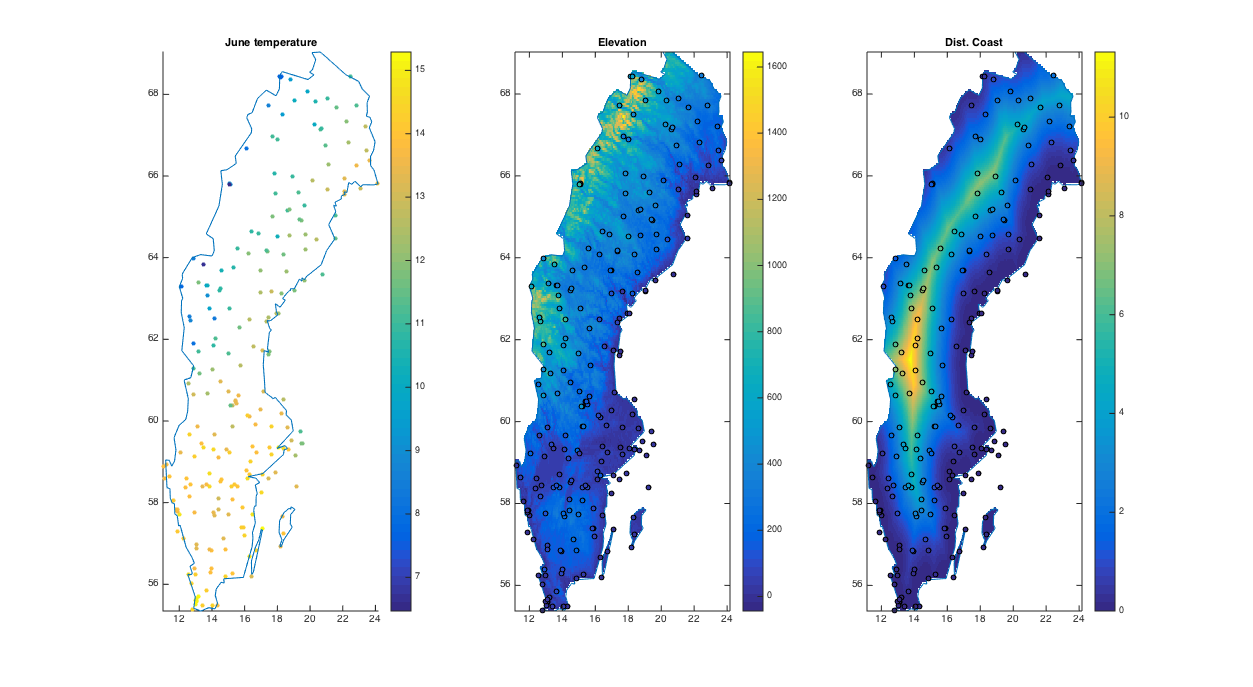
\includegraphics[width=0.8\linewidth]{raw_data_plot.png}
	\caption{Raw Data Plot...}
	\label{fig:rawdataplot}
\end{figure}
\subsection{Least-Squares}
The mean of the spatial data is modelled as a linear function of the covariates. Figure \ref{fig:covariates} shows a plot of the mean temperature (observations) as a function of the available covariates from the dataset {\texttt{SweObs}} containing the 250 measurements.
\begin{figure}[ht]
	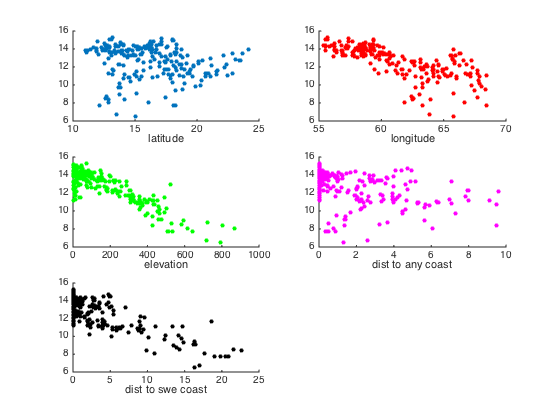
\includegraphics[width=0.8\linewidth]{covariates.png}
	\caption{Observation vs covariates}
	\label{fig:covariates}
\end{figure}
It was found that longitude does not relate linearly with the average temperatures measured and hence is left out of modelling. In order to select the appropriate covariates, we formed five models (A,B,C,D,E) containing different set of covariates as tabulated in Table \ref{tab:models}.
\begin{table}[H]
\centering
\begin{tabular}{lp{9cm}}
\hline
{\bf Model} & {\bf Covariates} \\
\hline
* A & Latitude, elevation, distance to any coast, distance to Swedish coast\\
 B & Latitude, elevation, distance to Swedish coast\\
 C & Latitude, elevation, distance to any coast\\
 D & Latitude, distance to any coast, distance to Swedish coast\\
 E & Latitude, elevation\\
\hline
\end{tabular}
\caption{Models and the respective covariates, with average temperature as the independent varible.}
\label{tab:models}
\end{table}
The standard errors of the residuals and the Akaike Information Criterion (AIC) seen in figure \ref{fig:modperf} shows that model A performs best.
\begin{figure}[ht]
\centering
  \subfloat[Std. Err of the residuals for each of the models.]{{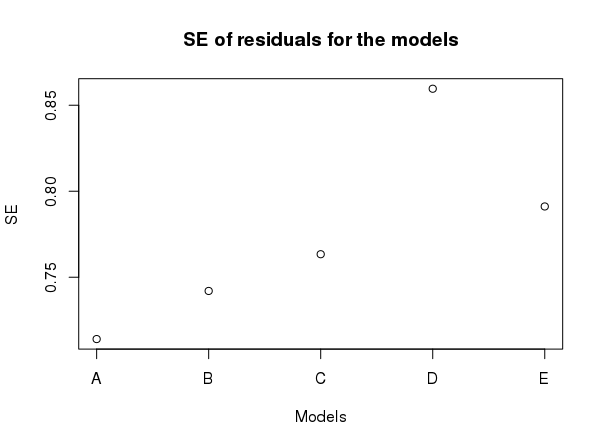
\includegraphics[width=5cm]{RSS_models.png} }}%
  \qquad
  \subfloat[AIC for each of the models.]{{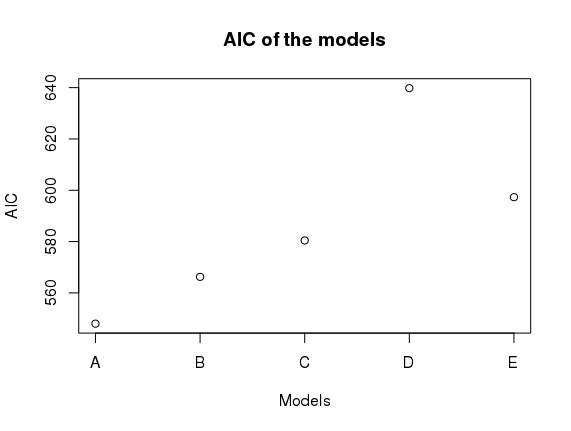
\includegraphics[width=5cm]{AIC_models.png} }}%
  \caption{Performance evaluation of the five models (A,B,C,D,E). Model A has the least std. error of the residuals and the best AIC metric.}
\label{fig:modperf}
\end{figure}

Thus, using model A, we may express the observed temperature $\bY$ as a linear function of latitude ($\bx_1$), elevation ($\bx_2$), distance to any coast ($\bx_3$) and the distance to Swedish coast ($\bx_4$).
\begin{align}
  \bY &\triangleq \bX \bbeta +  {\boldsymbol \epsilon}  \nonumber \\
   \bY &= \beta_0 + \beta_1 \bx_1 + \beta_2 \bx_2 + \beta_3 \bx_3 + + \beta_4 \bx_4 + {\boldsymbol \epsilon}
\end{align}
where $\beta_0$ is the intercept, $\beta_1 \dots \beta_4$ are the parameters and ${\boldsymbol \epsilon} \sim N(0,{\bf I})$. For  validation, 25 observations are set aside and we use $N = 225$ data points for the model parameter estimation. The estimated parameters are given by the least-squares solution $\hat \bbeta = (\bX^T \bX)^{-1} \bX^T \bY$. The estimated parameters (and their standard deviations ) are tabulated below.
\begin{table}[H]
\centering
\begin{tabular}{lcc}
\hline
{\bf Parameter} & {\bf Estimate} & {\bf SE }\\
\hline
$\hat \beta_0$ & 23.972 & 0.95 \\
$\hat \beta_1$ & -0.169 & 0.016\\
$\hat \beta_2$ & -0.005 & 0.0005 \\
$\hat \beta_3$ & 0.106 & 0.025\\
$\hat \beta_4$ & -0.089 & 0.015\\
\hline
\end{tabular}
\caption{Parameter Estimates and corresponding standard errors.}
\label{tab:olsest}
\end{table}
The variance of the residuals $\sigmaeps^2 = 0.48$. The mean temperatures at the validation points are given by
\begin{equation}
\bE(\hat \bY_v) = \bX_v \hat \bbeta
\end{equation}
where $\hat \bY_v$ denotes the average temperature estimates at the validation points, $\bX_v$  the regressor matrix formed using the latitude, elevation, distance to any coast and distance to Swedish coast of the 25 validation points and $\hat \bbeta$ the estimated model parameters. The variance and the 95\% confidence interval are given by
\begin{align*}
\bV(\hat \bY_v) &= \sigmaeps^2 (\bX_v (\bX_v^T\bX_v)^{-1} \bX_v^T + 1) \\
\text{CI, 95\%} &= \bE(\hat \bY_v) \pm 1.96 \text{ SE}(\hat \bY_v)
\end{align*}
where $\text{SE}(\hat \bY_v) = \sqrt{\bV(\hat \bY_v)}$. Figure \ref{fig:olsresults} shows a plot of prediction and confidence intervals for the validation points and also the predictions for the {\texttt{SweGrid}} data along with the corresponding standard error.
\begin{figure}[ht]
\centering
  \subfloat[]{{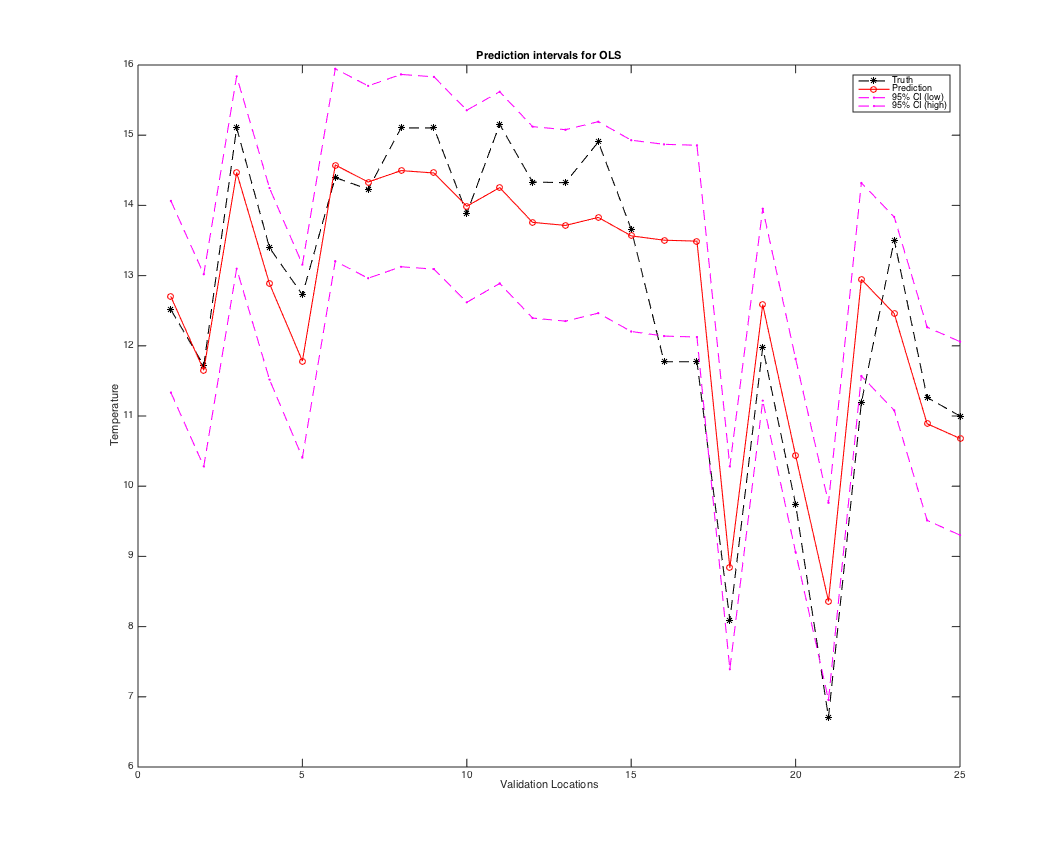
\includegraphics[width=4.5cm]{ols_valdat_pred_ci.png} }}%
  \qquad
  \subfloat[]{{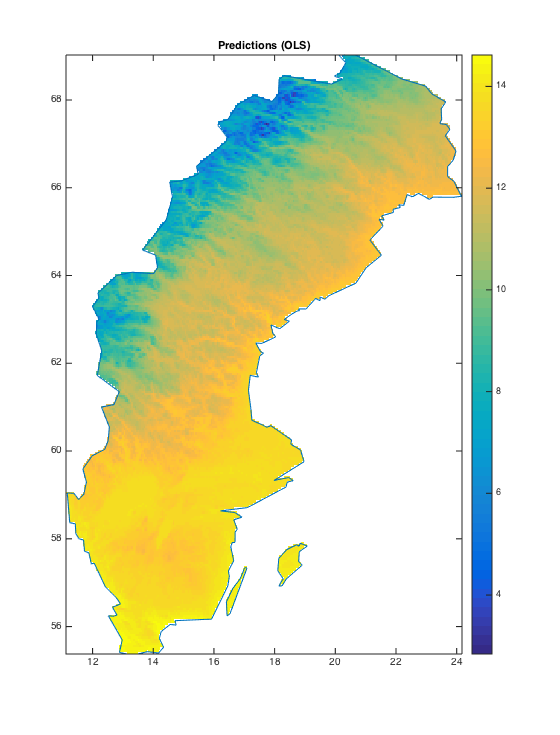
\includegraphics[width=2.8cm]{pred_ols_grid.png} }}%
  \qquad
  \subfloat[]{{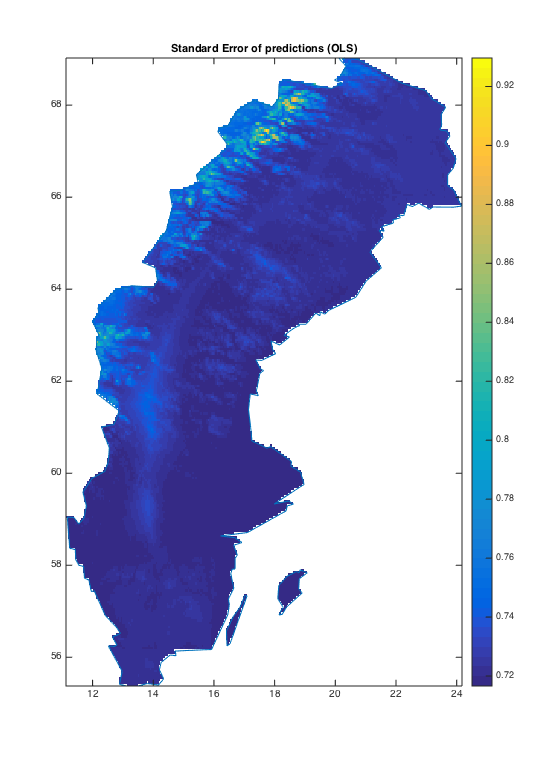
\includegraphics[width=2.8cm]{se_pred_ols.png} }}%
  \caption{(a): Estimate and confidence intervals (95\%) for the 25 validation points. (b),(c): Predictions and SE of predictions for \texttt{SweGrid} data.}
\label{fig:olsresults}
\end{figure}

\subsection{Universal Kriging}

\section{Conclusions}

\end{document}
